\documentclass[12pt]{article}
	
\usepackage[margin=1in]{geometry}		% For setting margins
\usepackage{amsmath}				% For Math
\usepackage{fancyhdr}				% For fancy header/footer
\usepackage{graphicx}				% For including figure/image
\usepackage{cancel}				% To use the slash to cancel out stuff in work
\usepackage[spanish]{babel}
\usepackage{hyperref}
\usepackage{enumitem}
\usepackage{float}
\usepackage[utf8]{inputenc}

%%%%%%%%%%%%%%%%%%%%%%
% Set up fancy header/footer
\pagestyle{fancy}
\fancyhead[LO,L]{Base de Datos}
\fancyhead[CO,C]{SIA 301 - Passwords in SQL}
\fancyhead[RO,R]{29 de septiembre de 2023}
\fancyfoot[LO,L]{}
\fancyfoot[CO,C]{\thepage}
\fancyfoot[RO,R]{}
\renewcommand{\headrulewidth}{0.4pt}
\renewcommand{\footrulewidth}{0.4pt}
% secciones con 0.1
%\renewcommand{\thesection}{0.\arabic{section}}
%%%%%%%%%%%%%%%%%%%%%%

\begin{document}
% PLANTILLA INICIAL
\noindent \textbf{Universidad Nacional del Altiplano\\
Docente: } Fred Torres Cruz\\
\textbf{Estudiante:} Maye Mamani Victor Raul

\vspace{2mm}
\noindent\textbf{Trabajo Encargado N°6}\\
% %%%%%%%%%%%%%%%%%%%%%%%%%%%%%%%%%%%%%%%%%%%%%%%%%%
%%%%%%%%%%%%%%%%%%%%%%%%%%%%%%%%%%%%%%%%%%%%%%%%%%%%%

%%%%%%%%%% CONTENIDO DE LA TAREA
%%%%%%%%%%%%%%%%%%%%%%%%%%%%%%%%%%%%
%%%%%%%%%%%%%%%%%%%%%%%%%%%%%%%%%%%%%%%%%%%%%%%
%%%%%%%%%%%%%%%%%%%%%%%%%%%%%%%%%%%%%%%%%%%%%%%%%%%%%%%%%%%%%%%

\section{Interfaz de usuario para el login y registro de usuarios}

\begin{figure}[H]
    \centering
    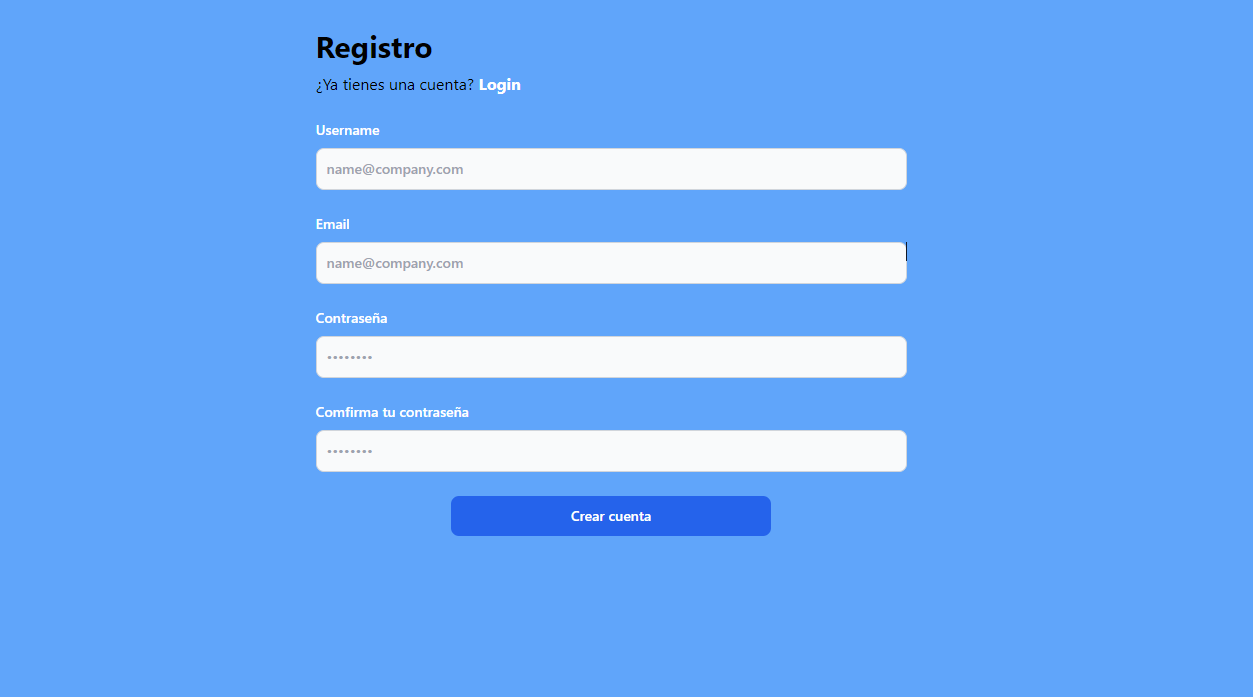
\includegraphics[width=1\textwidth]{./img/UI-Register.png}
    \caption{Interfaz de usuario para el registro de usuarios}
    \label{fig:my_label}
\end{figure}

\begin{figure}[H]
    \centering
    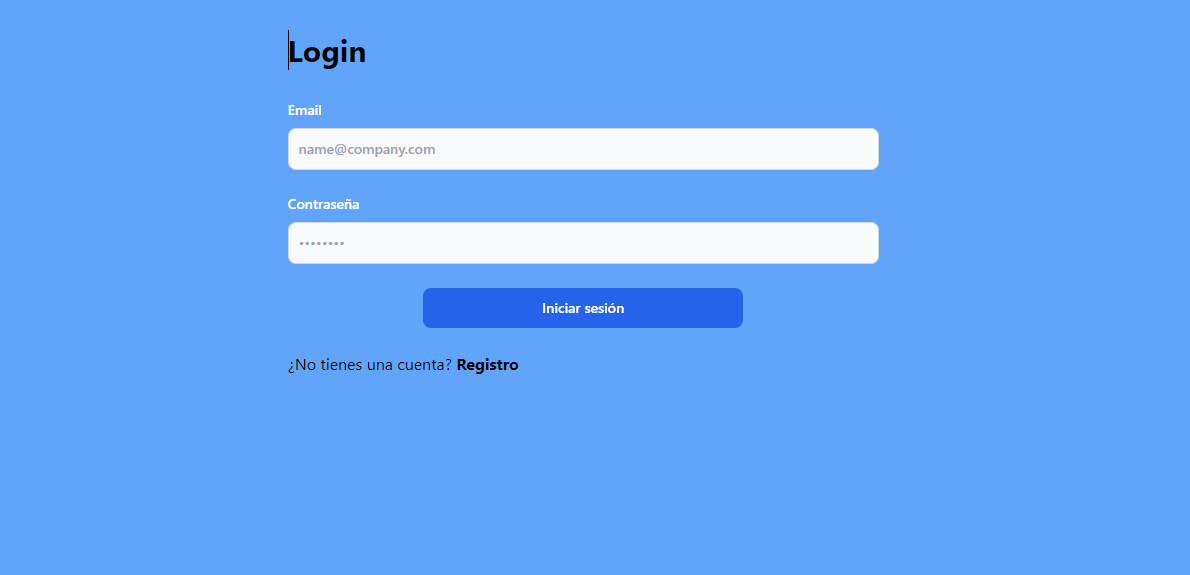
\includegraphics[width=1\textwidth]{./img/UI-Login.png}
    \caption{Interfaz de usuario para el login de usuarios}
    \label{fig:my_label}
\end{figure}

%%%%%%%%%%%%%%%%%%%%%%%%%%%%%%%%%%%%%%%%%%%%%%%%%%%%

\section{Ejemplo de uso del registro de usuarios}
\begin{figure}[H]
    \centering
    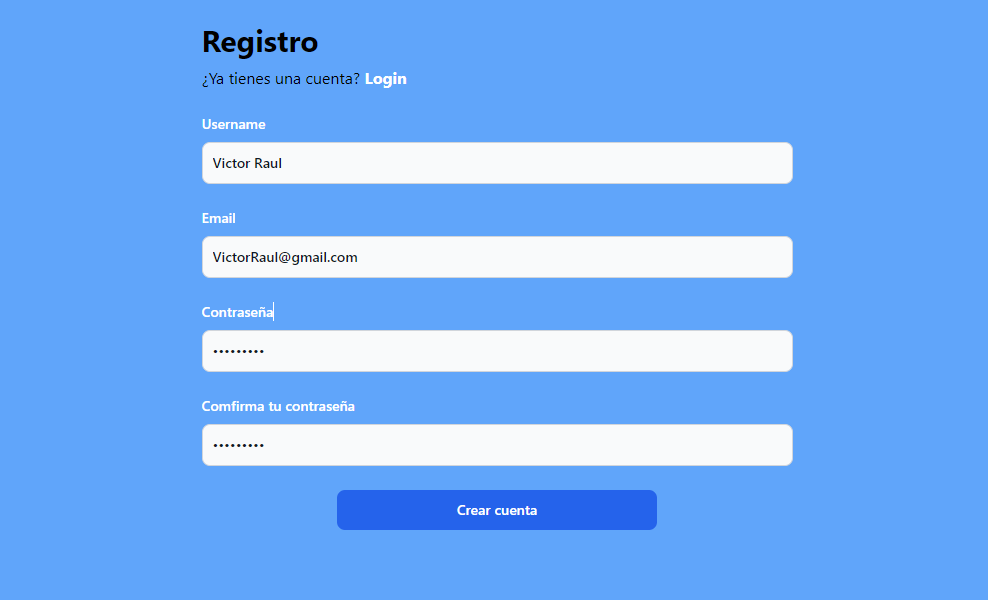
\includegraphics[width=0.9\textwidth]{./img/Register-example.png}
    \caption{Ejemplo de uso del registro de usuarios}
    \label{fig:my_label}
\end{figure}

\begin{figure}[H]
    \centering
    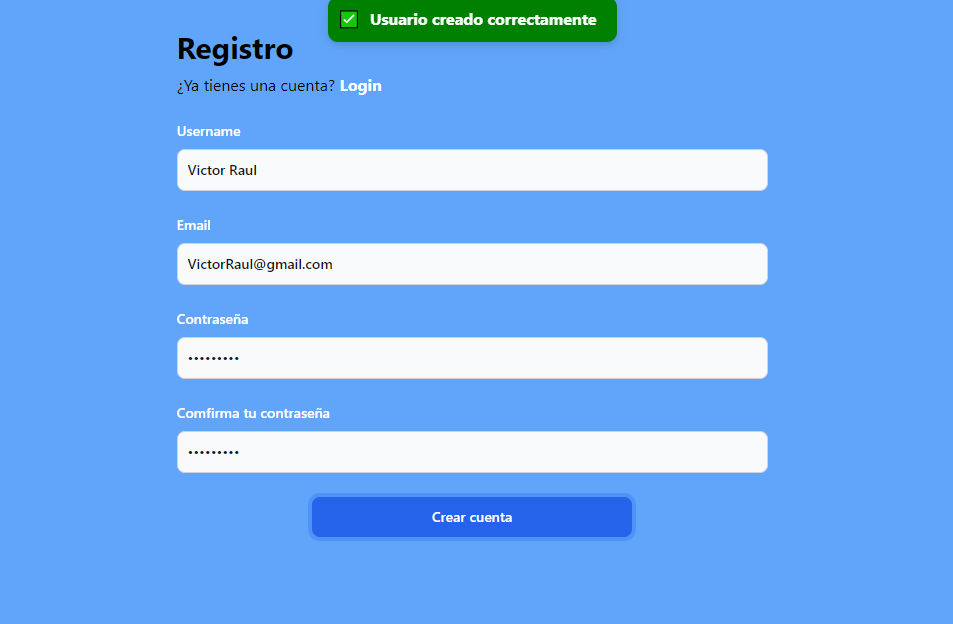
\includegraphics[width=0.9\textwidth]{./img/Register-successfully.png}
    \caption{Registro exitoso de usuario}
    \label{fig:my_label}
\end{figure}



%%%%%%%%%%%%%%%%%%%%%%%%%%%%%%%%%%%%%%%%%%%%%%%%%

\section{Ejemplo de uso del login de usuarios}
\begin{figure}[H]
    \centering
    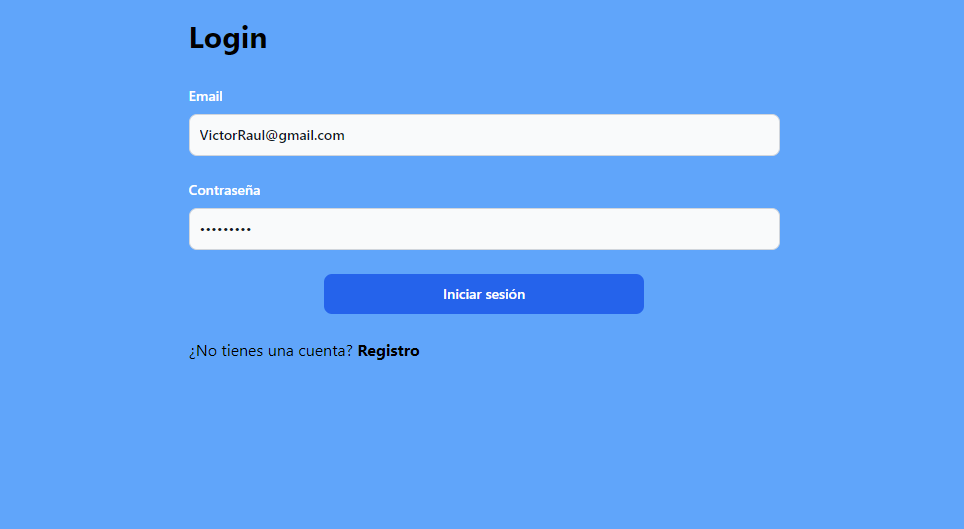
\includegraphics[width=1\textwidth]{./img/Login-example.png}
    \caption{Ejemplo de uso del login de usuarios}
    \label{fig:my_label}
\end{figure}

\begin{figure}[H]
    \centering
    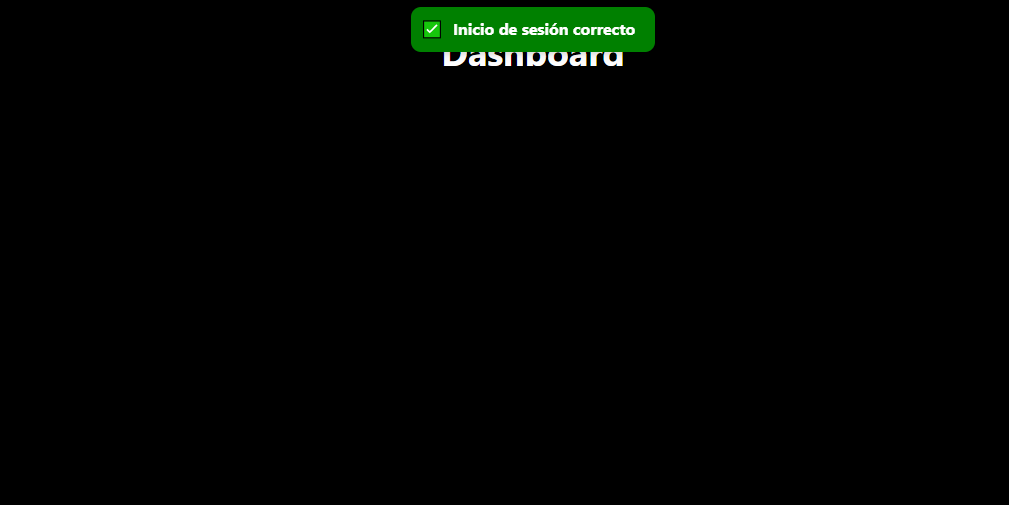
\includegraphics[width=1\textwidth]{./img/Login-successfully.png}
    \caption{Login exitoso de usuario}
    \label{fig:my_label}
\end{figure}




\section{Base de datos en MongoDB}
\begin{figure}[H]
    \centering
    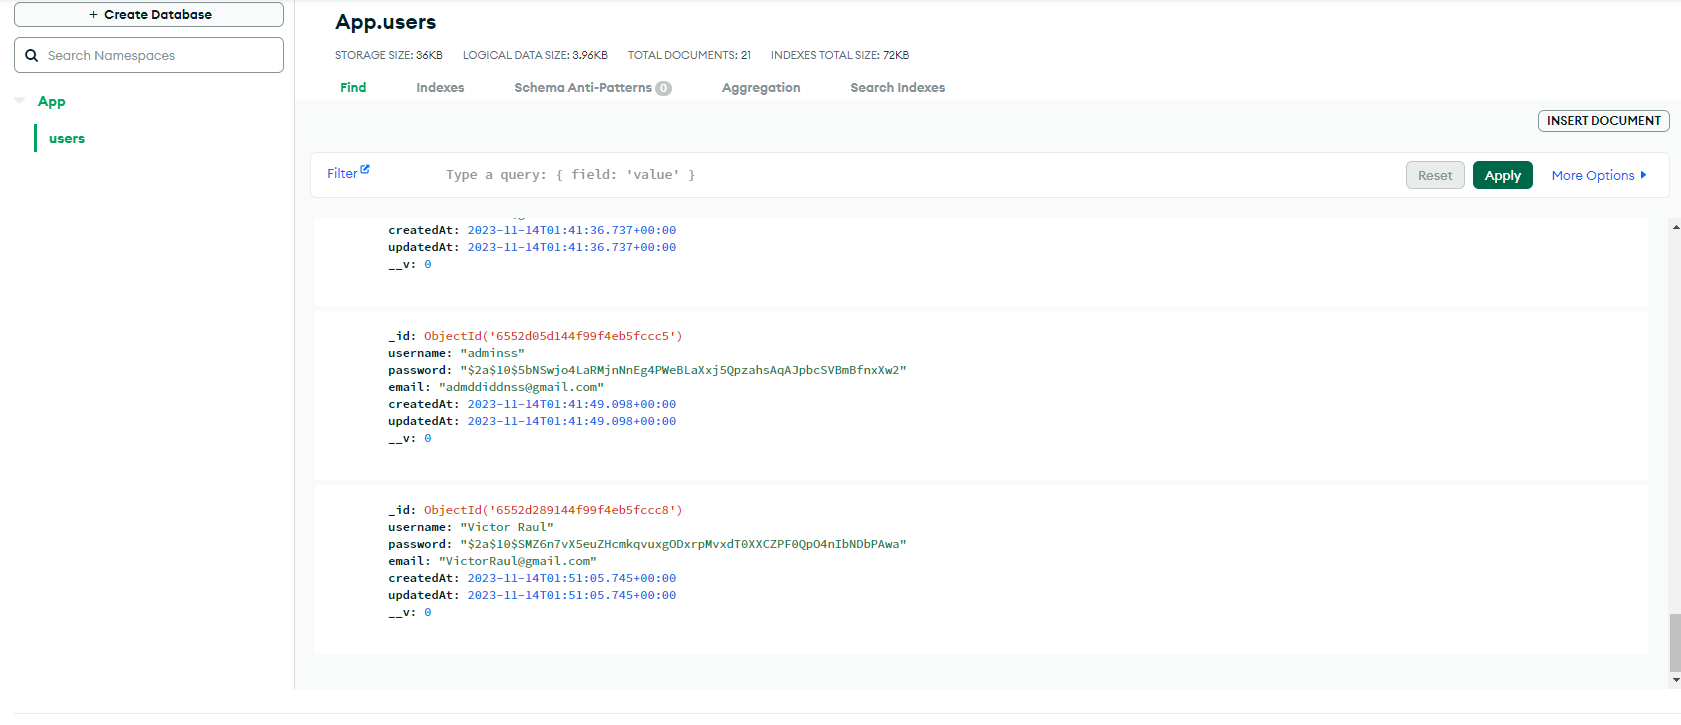
\includegraphics[width=1\textwidth]{./img/DB-MongoDB.png}
    \caption{Base de datos en MongoDB}
    \label{fig:my_label}
\end{figure}
\section{Codigo SQL de la base de datos (MONGODB)}

\large{Use MongoDB por lo que no use SQL, pero de todas formas dejo el codigo SQL que hubiera usado}

\large{Crear base de datos}
\begin{verbatim}
    CREATE DATABASE App;
    USE App;
\end{verbatim}

\large{Crear tabla}

\begin{verbatim}
    CREATE TABLE Users (
    id INT AUTO_INCREMENT PRIMARY KEY,
    username VARCHAR(255) NOT NULL,
    password VARCHAR(255) NOT NULL,
    email VARCHAR(255) NOT NULL UNIQUE,
    created_at TIMESTAMP DEFAULT CURRENT_TIMESTAMP,
    updated_at TIMESTAMP DEFAULT CURRENT_TIMESTAMP ON UPDATE CURRENT_TIMESTAMP
    );

\end{verbatim}
\large{Insertar datos}
\begin{verbatim}
    INSERT INTO Users (username, password, email) 
    VALUES ('Victor', '123456', 'victor@gmail.com');
\end{verbatim}

\section{Codigo fuente de la interfaz de usuario}

% link
\large \textbf{Link:}
\url{https://github.com/valec3/Login-Register-MERN}

%%%%%%%%%%%%%%%%%%%%%%%%%%%%%%%%%%%%%%%%%%%%%%%%%%%%%%%%%%%%%%
%%%%%%%%%%%%%%%%%%%%%%%%%%%%%%%%%%%%%%%%%%%%%%%%%%
%%%%%%%%%%%%%%%%%%%%%%%%%%%%%%%%%%%%
%%%%%%%%%% FIN TAREA



\end{document}


% PLANTILLA PARA IMAGENES
% 
% \begin{figure}[h]
%       \centering
%       \includegraphics[width=1\textwidth]{show-facu-update.jpg}
%       \caption{Facultad actualizada con exito}
%       \label{fig:mi_imagen}
%     \end{figure}